%%%%%%%%%%%%%%%%%%%%%%%%%%%%%%%%%%%%%%%%%%%%%%%%%%%%%%%%%%%%%%%%%%%%%%%
% Based on IEEE the conference template available                     %
% at https://www.ieee.org/conferences/publishing/templates.html       %
% Adapted for the Data Science Lab course at Politecnico di Torino    %
% by Giuseppe Attanasio, Flavio Giobergia                             %
% 2020, DataBase and Data Mining Group                                %
%%%%%%%%%%%%%%%%%%%%%%%%%%%%%%%%%%%%%%%%%%%%%%%%%%%%%%%%%%%%%%%%%%%%%%%

\documentclass[conference]{IEEEtran}
\usepackage{cite}
\usepackage{amsmath,amssymb,amsfonts}
\usepackage{algorithm}
\usepackage{algorithmic}
\usepackage{graphicx}
\usepackage{textcomp}
\usepackage{xcolor}
\usepackage{subfigure}

\begin{document}

\title{
Lab L7: Epidemic processes
}

\author{
    \IEEEauthorblockN{Emanuele Pietropaolo}
    \IEEEauthorblockA{
        \textit{Politecnico di Torino} \\
        Student id: s319501 \\
        emanuele.pietropaolo@studenti.polito.it
        }
}

\maketitle
% \begin{abstract}
    
% \end{abstract}

\section{Problem overview}

The SIR model is a compartmental model that divide a population into three compartments: Susceptible individuals, Infectious individuals, Removed individuals.
%
This is well suited to the task of simulating epidemic processes.
%
It can also be extended to include other categories (such as deaths, recovered and quarantined).

This paper presents a simulation of an SIR model to study the effect of a virus containment strategy.
%
The SIR model used in this simulation has $7$ compartments: 
\begin{itemize}
    \item Susceptible
    \item Infectious
    \item Quarantined
    \item Recovered
    \item Hospitalized
    \item Intensive treatment
    \item Deaths
\end{itemize}

\section{Proposed approach}

The event in which a susceptible individual comes into contact with the epidemic and becomes infectious, the event in which an infectious individual is quarantined and the event in which an infectious individual becomes a recovered/dead individual are simulated as Hawkes processes.
%
According to the formulas:

\begin{center}
    \begin{math}
        \lambda_{S->I}(t|H_t) = \lambda S(t) I(t)
    \end{math}
\end{center}

\begin{center}
    \begin{math}
        \lambda_{I->R}(t|H_t) = \gamma I(t)
    \end{math}    
\end{center}

\begin{center}
    \begin{math}
        \lambda_{I->Q}(t|H_t) = \gamma_Q I(t)
    \end{math}    
\end{center}

\begin{center}
    \begin{math}
        \lambda_{Q->R}(t|H_t) = \gamma Q(t)
    \end{math}    
\end{center}

The point processes are generated accordingly to the thinning algorithm.

A further simulation is then carried out using ODA's formulae to confront the stochastic result.
%
Both simulations take into account the situation of saturation of space in hospitals and intensive care units.

\subsection{Proposed strategy}

The proposed strategy involved a quarantine period regulated by a specific gamma parameter ($\gamma_Q$).
%
This simulates the situation in which the government imposes that an infectious individual does not spread the virus.

Another measure my simulation deals with is the one where the government restricts freedom of movement to limit the spread of the virus. 
%
This action is taken based on the availability in the hospital department.
%
When the number of available places go over $30\%$ of the total the first measure are taken.
%
The second measure is taken when the number goes over $50\%$.
   
\section{Results}

\begin{figure}[!ht]
    \centering
    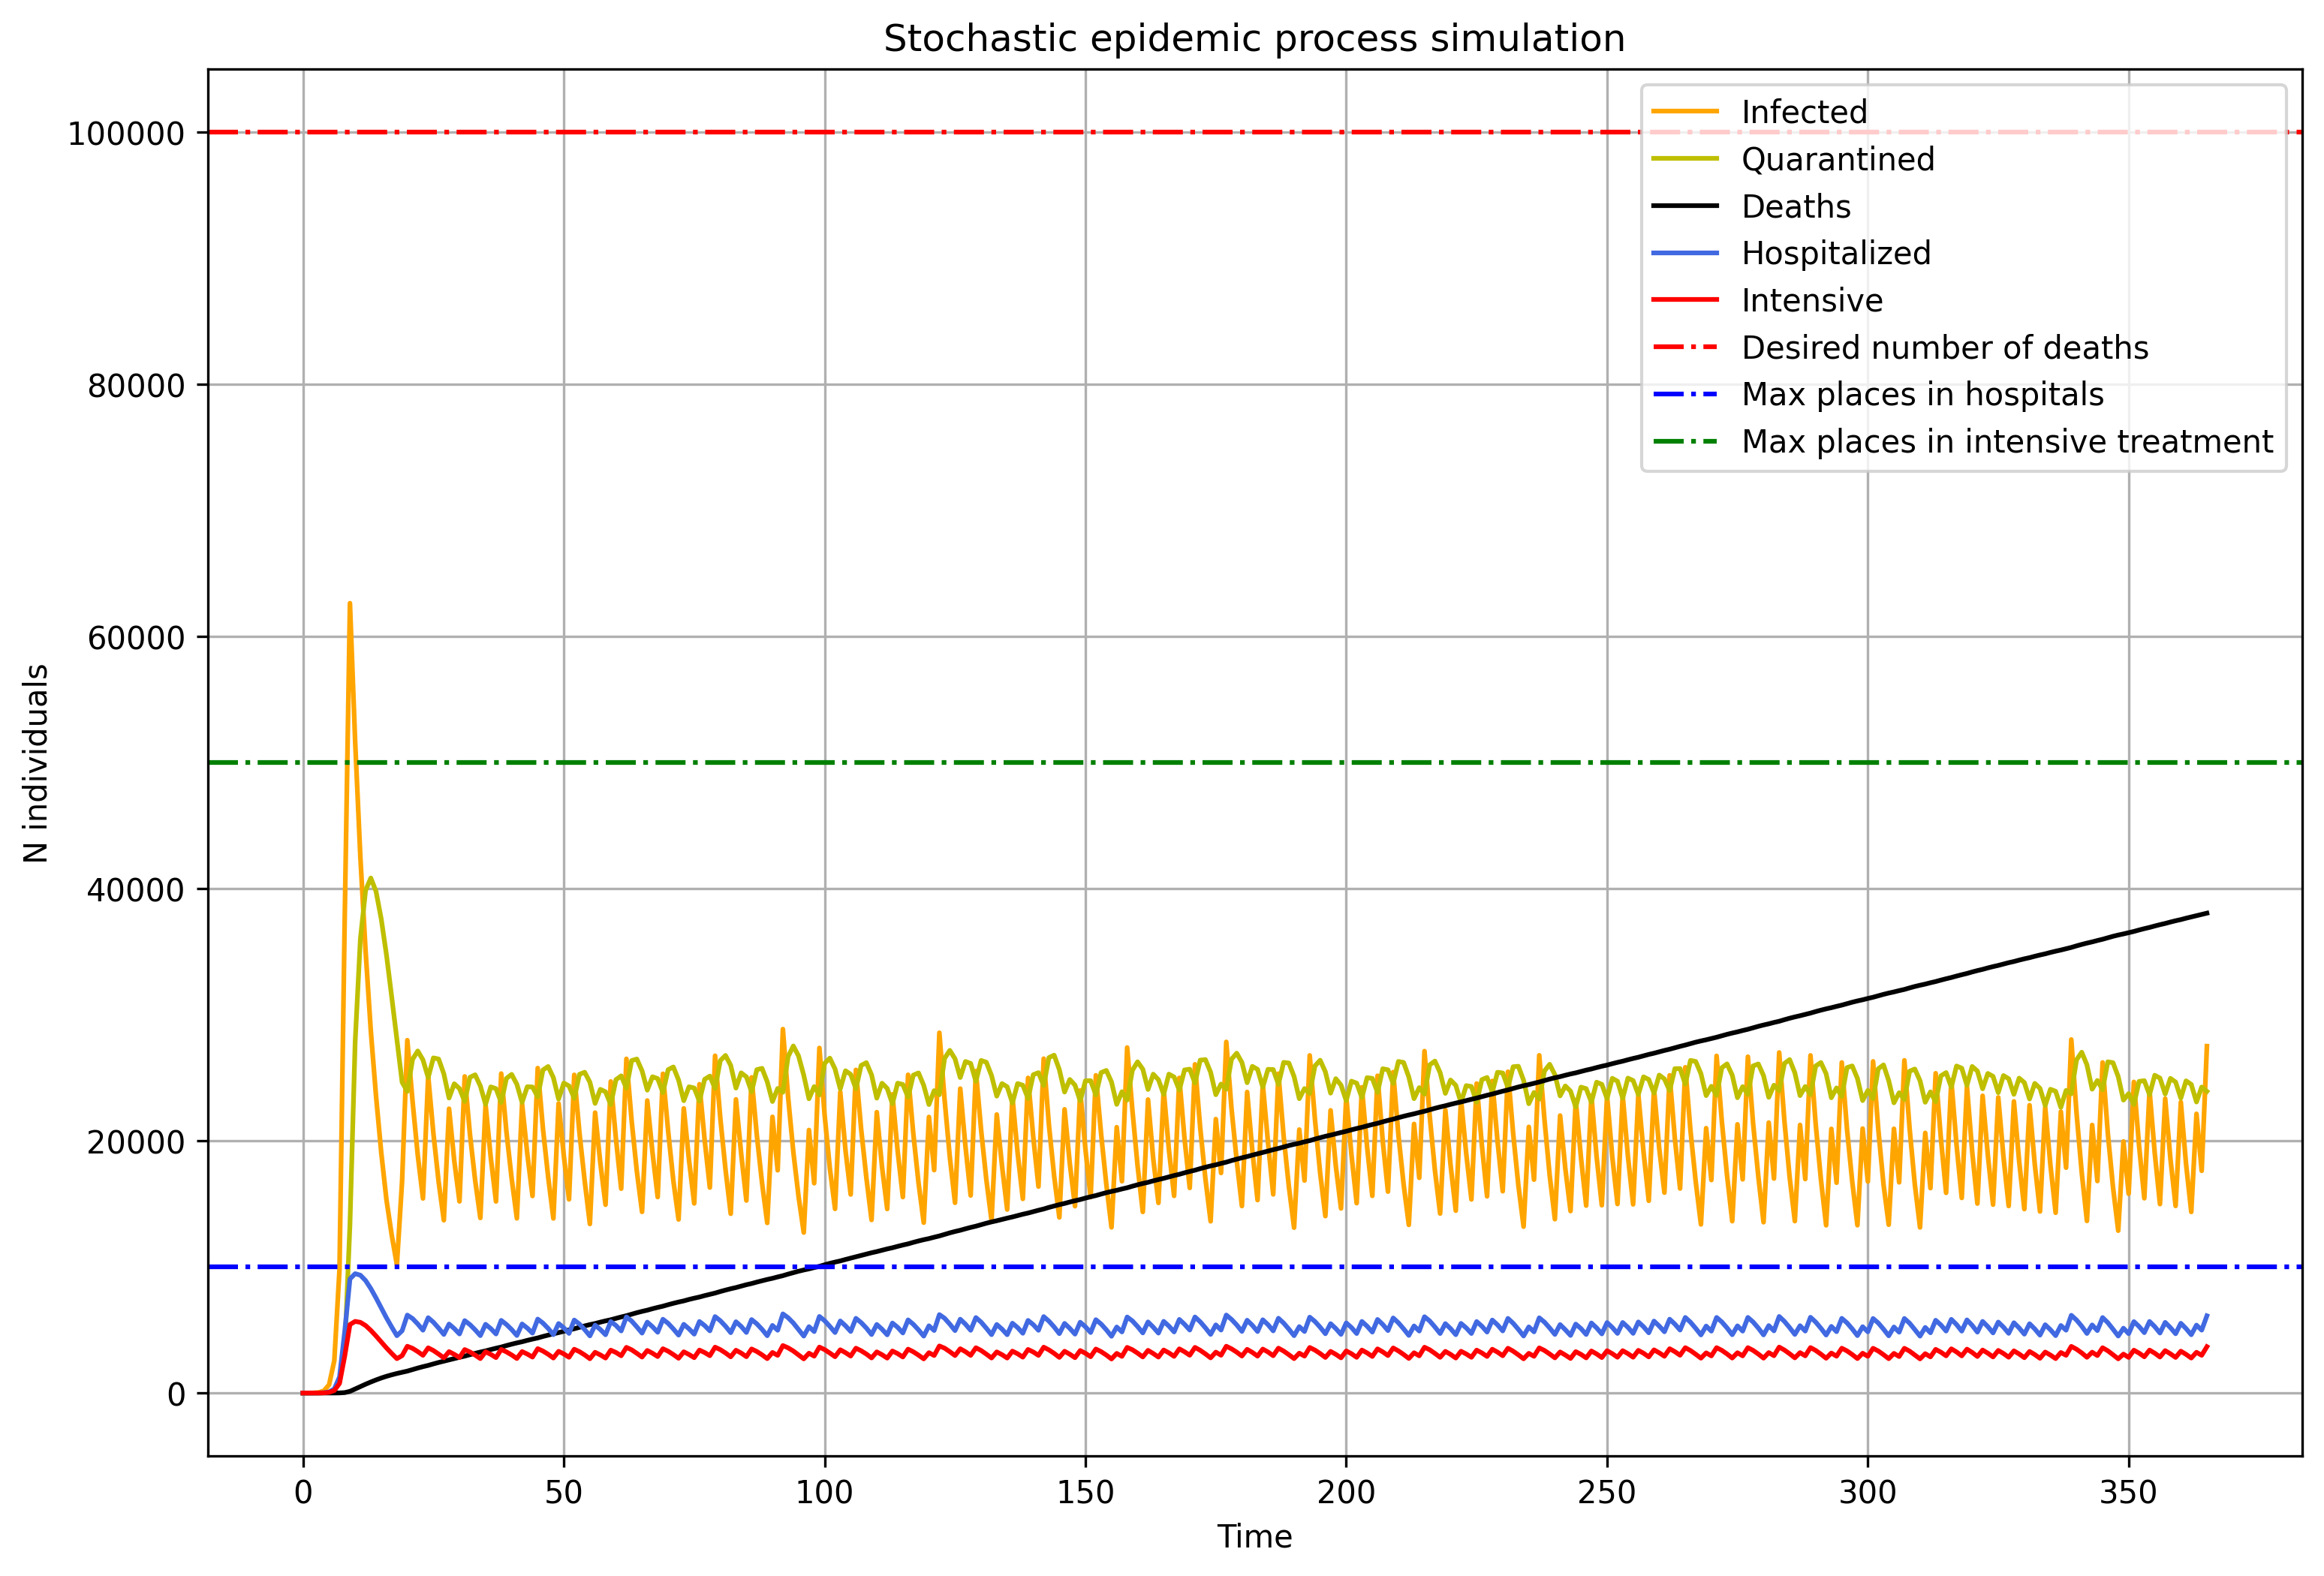
\includegraphics[width=\columnwidth]{media/stochastic.png}
    \caption[short]{Results for the stochastic simulation}
    \label{fig:stochastic}
\end{figure}

As shown in Fig.\ref{fig:stochastic} the proposed strategy successfully reduce the number of deaths under the desired threshold. Fig.\ref{fig:mean_field} confirms the results obtained with the stochastic simulation. 

\begin{figure}[!ht]
    \centering
    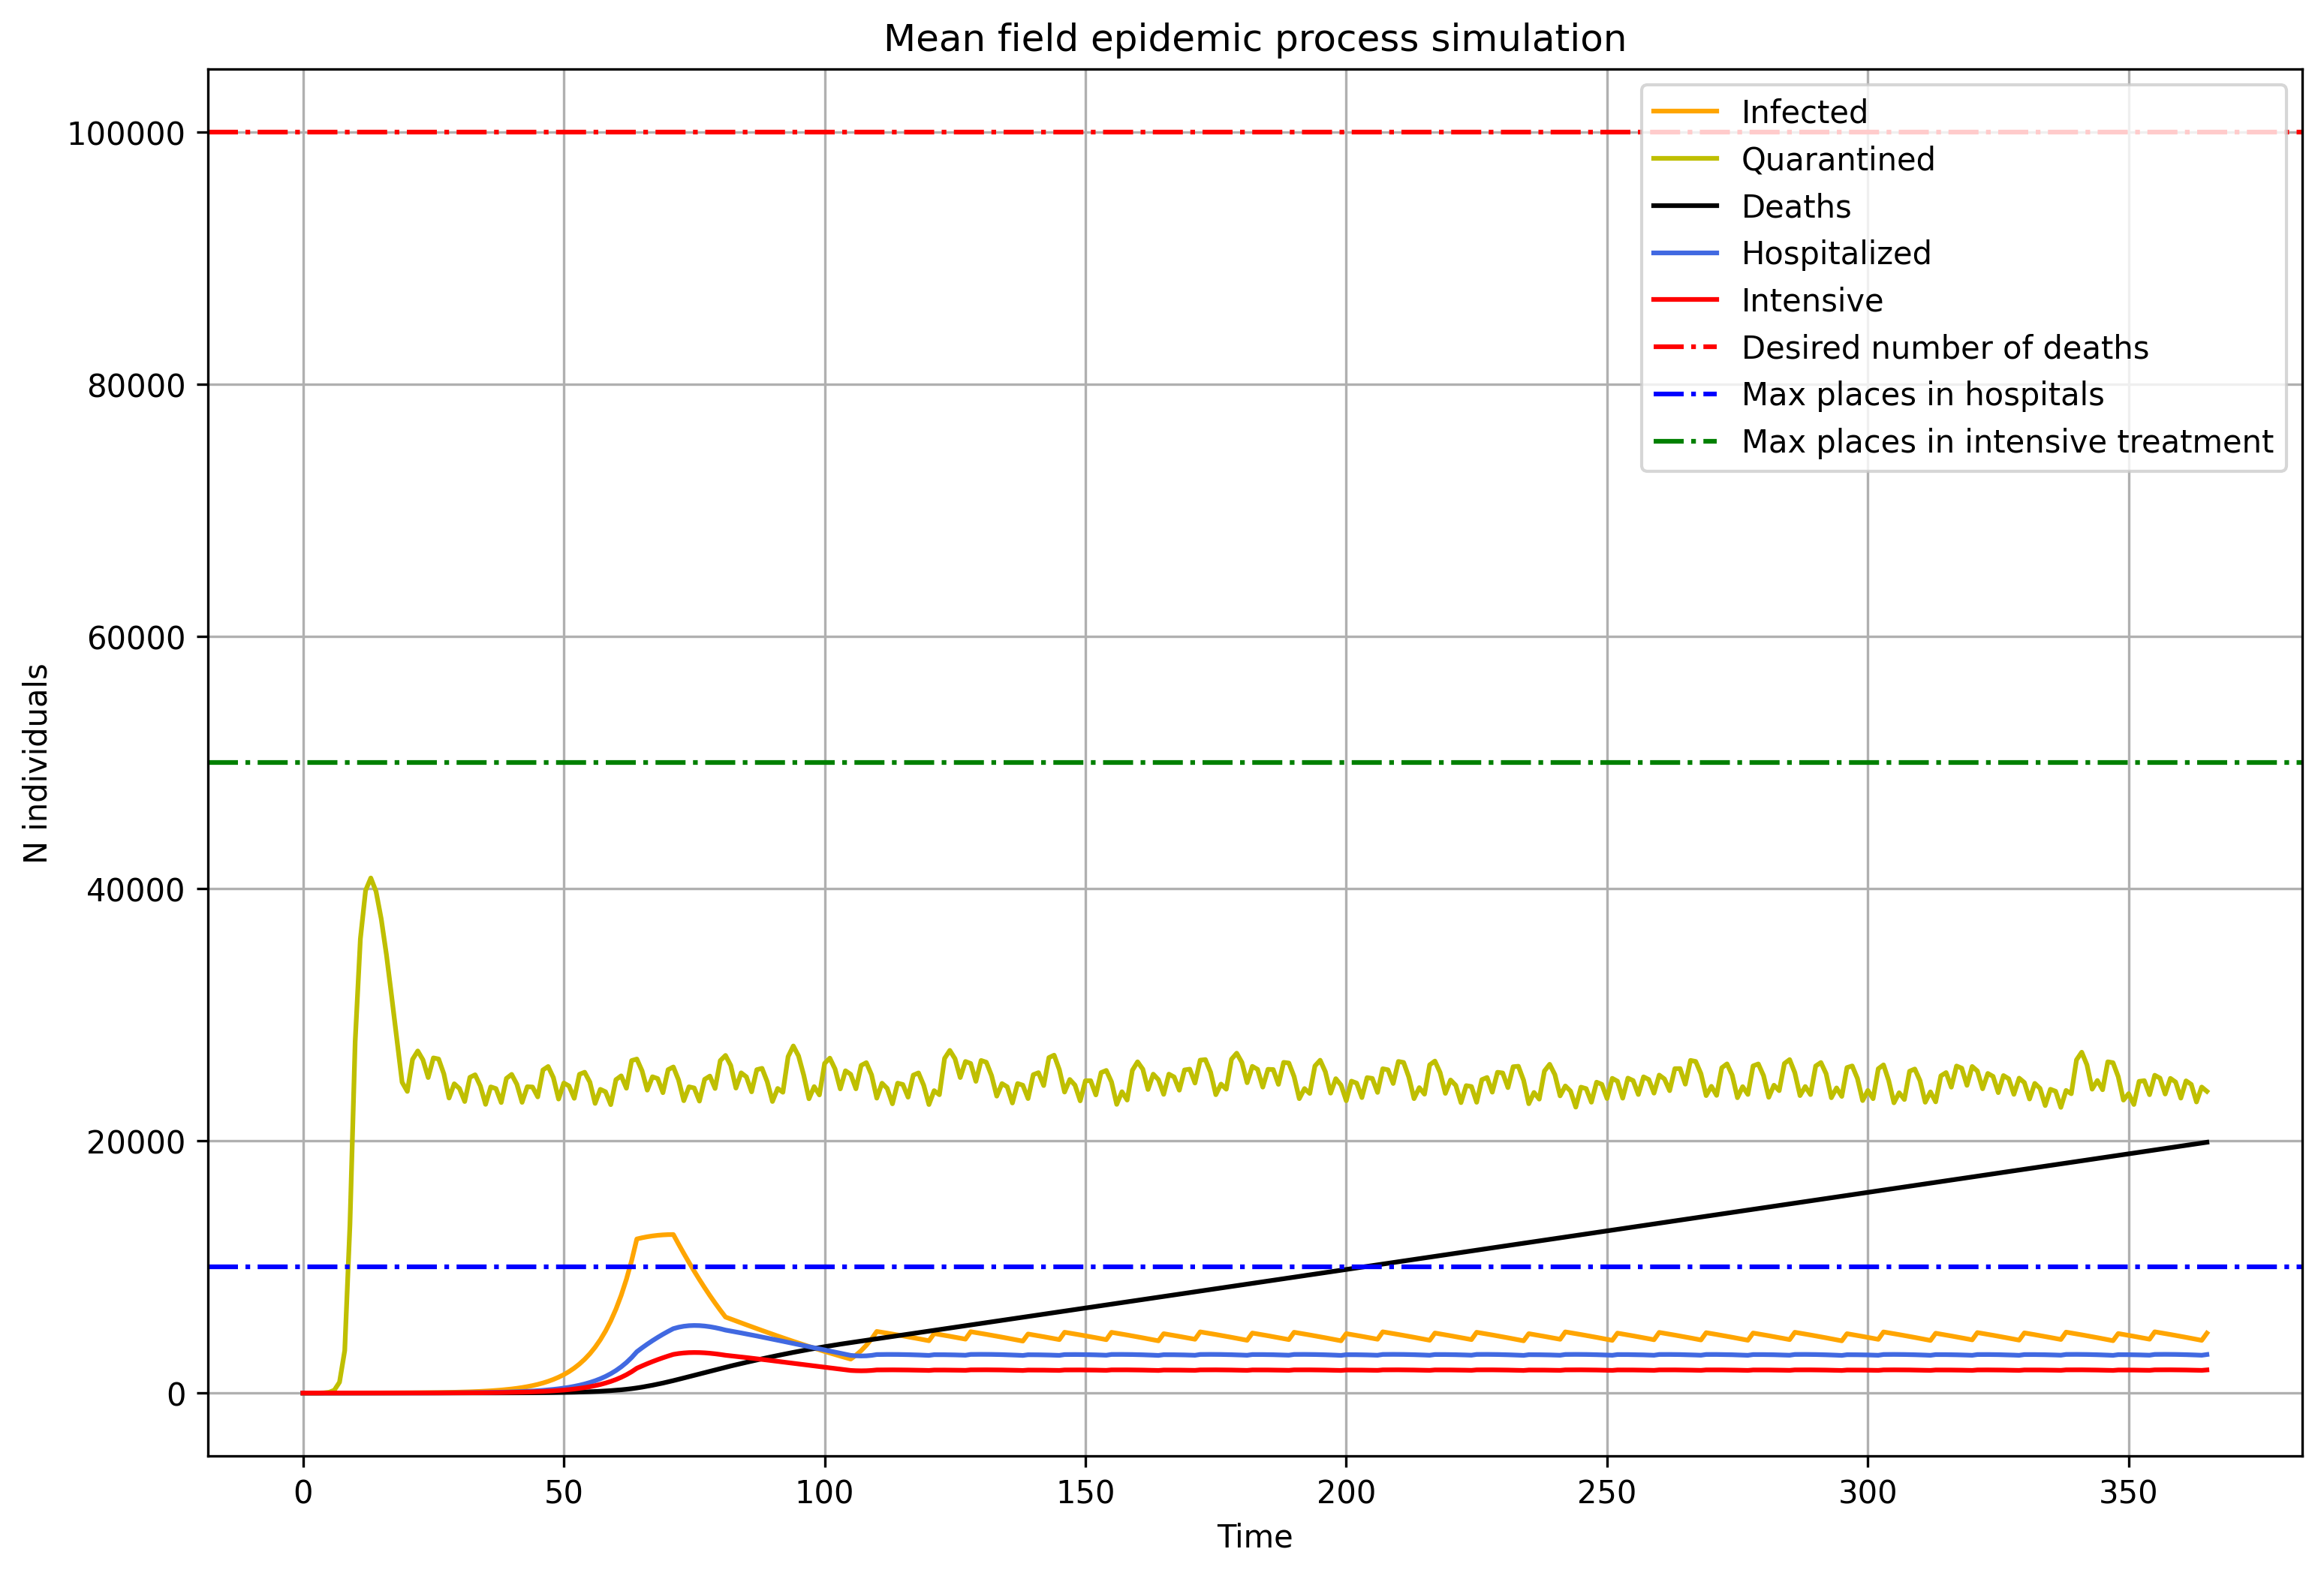
\includegraphics[width=\columnwidth]{media/mean_field.png}
    \caption[short]{Results for the mean field simulation}
    \label{fig:mean_field}
\end{figure}

There are interesting differences between the stochastic and mean field simulations. 
%
The two differ in the randomness and variability of the values.
%
In the second simulation there is an initial effect caused by the quarantined individuals.
%
They were a brake on the virus' progress. 
%
In the first case there is no evidence of this maybe due to generation of the random point process. 

%\bibliography{bibliography}
%\bibliographystyle{ieeetr}

\end{document}
